% !TEX root = ../main.tex
\section{The Continent} \label{sec::continent}

\DndDropCapLine{A}{ landmass so vast it houses all}
sorts of climates and biomes, Yuadrem is a supercontinent of impressive variety.
Many creatures of many natures interact with one another in its grounds, creating complex and diverse ecosystems and cultures.

Before any creature lived on the planet, the continent rose from the deepest of waters and established itself as a land amidst four violent seas.
It later became the cradle of civilization.
No matter how much change its inhabitants suffer, Yuadrem continues to stand as a testimony of the resilience of the ground, impervious to the business of its dwellers.

To distinguish its territories, Yuadrem is commonly divided into six regions: The Northern Territories, the Three Deserts, the Whaler's Sea, the Beryl Sea, the Barbaric Territories, and the Wildlands.

% !TEX root = ../main.tex

\begin{table*}[b]%
    \begin{DndTable}[width=\linewidth]{X}
        \centering
        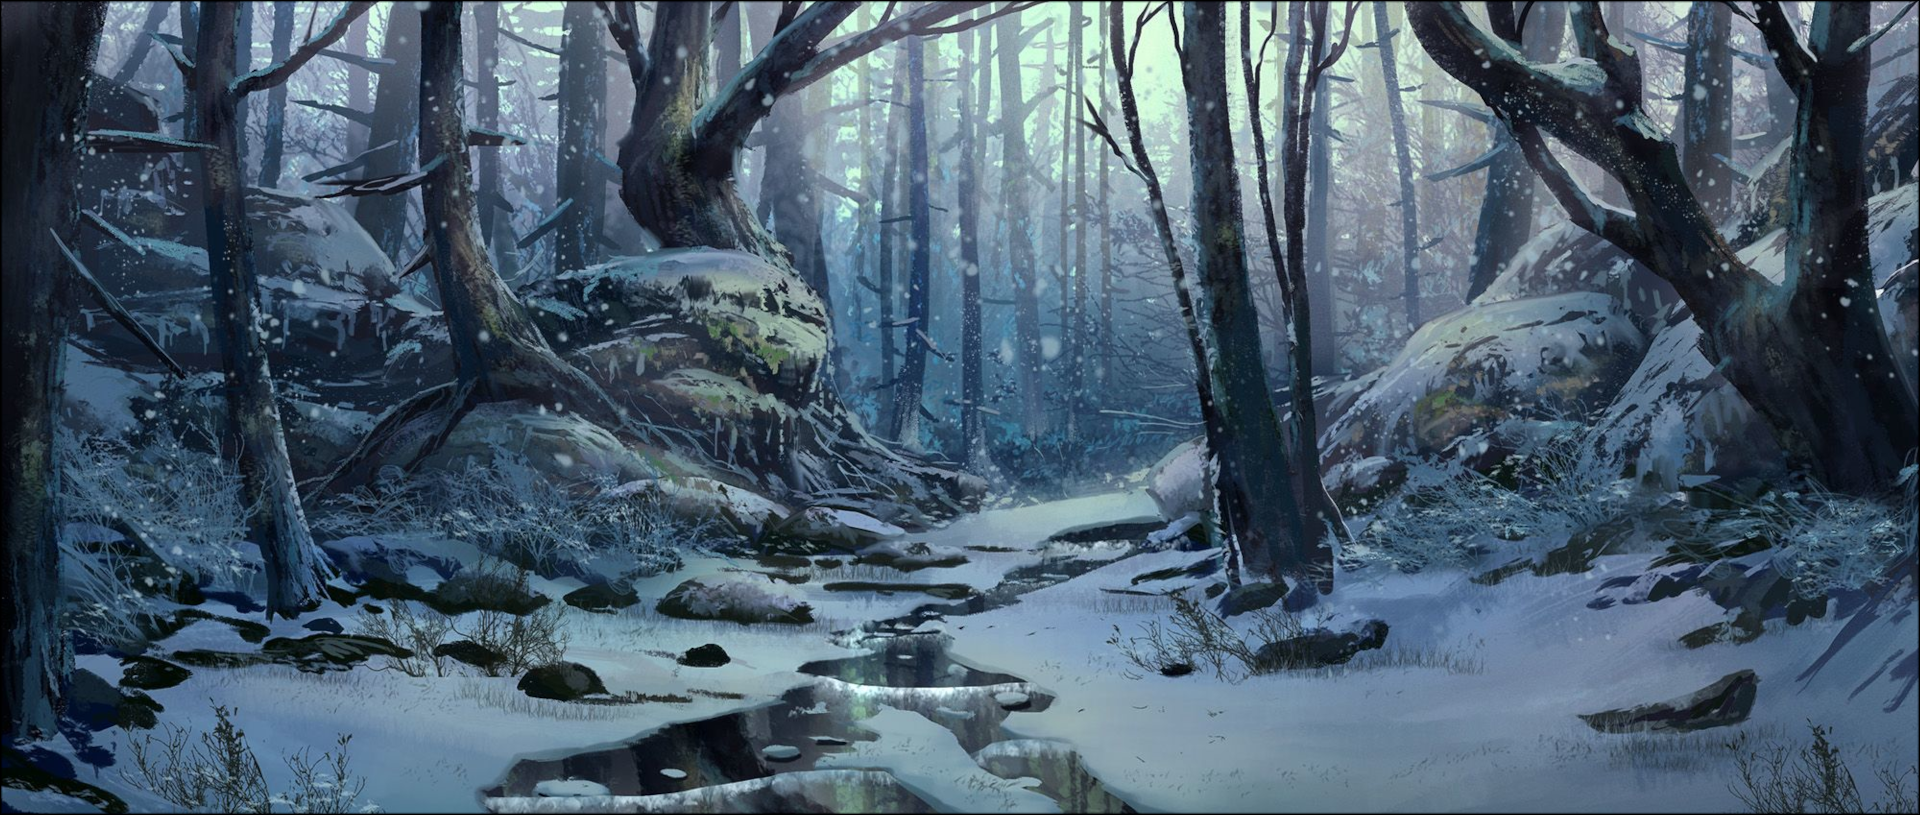
\includegraphics[width=0.95\textwidth]{01yuadrem/img/11tallwoods.png} \
        \centering \large{\textbf{The Tallwoods}}
    \end{DndTable}
\end{table*}

\subsection*{Northern Territories} \label{ssec::northernterritories}
The northmost region of Yuadrem, the Northern Territories are comprised by the Whitenorth, the Red Islands, the Tallwoods, the Blank Fields, and the Sulfur Lake.
The region is split by the Wall of Ice and Stone, a colossal mountain range that spans from coast to coast.

North of the wall is Whitenorth, an area split between the ancient ird kingdom of Krudzal and the territorial giants of Jatuunsa.
Its few inhabitants are beings of extreme resilience and fierceness, acclimated to the harsh habitat.
First among these are the giants, mountain-sized creature of stone, ever locked in war with Krudzal.

The middle of the region is characterized by the endless mists.
The area coincides with the north pole, and is inexplicably warm and misty despite its location.

To the west of Whitenorth is the Red Fjord, named so by its most common tree, the red maple.
The are is regarded sacred by the Krudzalians, who believe it to be the resting place of the sun god, Jua\~nanisz.
The fjord is currently occupied by Ribinhep, a uman nation ever standing up against the northerner irds.

Below the Wall of Ice and Stone are the Tallwoods and the Blank Fields.
The Tallwoods are an association of pine and redwood forest, using the mountains to hide from the cold winds.
The forests are devoid of civilized life, and the stone trolls who inhabit them make sure that they stay that way.

The Blank Fields are a vast, freezing tundra.
The low temperatures and strong winds in the area prohibit the growth of any vegetation.

The west of the fields are known as the Wurmlands, and they are solely inhabited by wurms.
Wurms are large reptile-like creatures that attack all foolish enough to approach their subterranean colonies.
The eastern portion of the land is filled to the brim with a variety of bughna gat tribes, ever in conflict for the large reserves of copper and coal in the mountains.

East to the fields is the Arctic Archipelago.
This cluster of islands separate the Whaler's Sea from the frigid ocean up north.
Mostly bare and desolate, the islets equally house ird, gat, uman, and zaloth settlements.

The strongest force in the archipelago is the Kaldrathal nation.
Having the only vessels strong enough to withstand the ship-sinking idzels, they regulate commerce in the entire archipelago.
% idzels or idzelal are inspired on Illhevi (https://abookofcreatures.com/category/iceland/page/2/).

% !TEX root = ../main.tex

% \begin{table*}[b]%
%     \begin{DndTable}[width=\linewidth]{X}
%         \centering
%         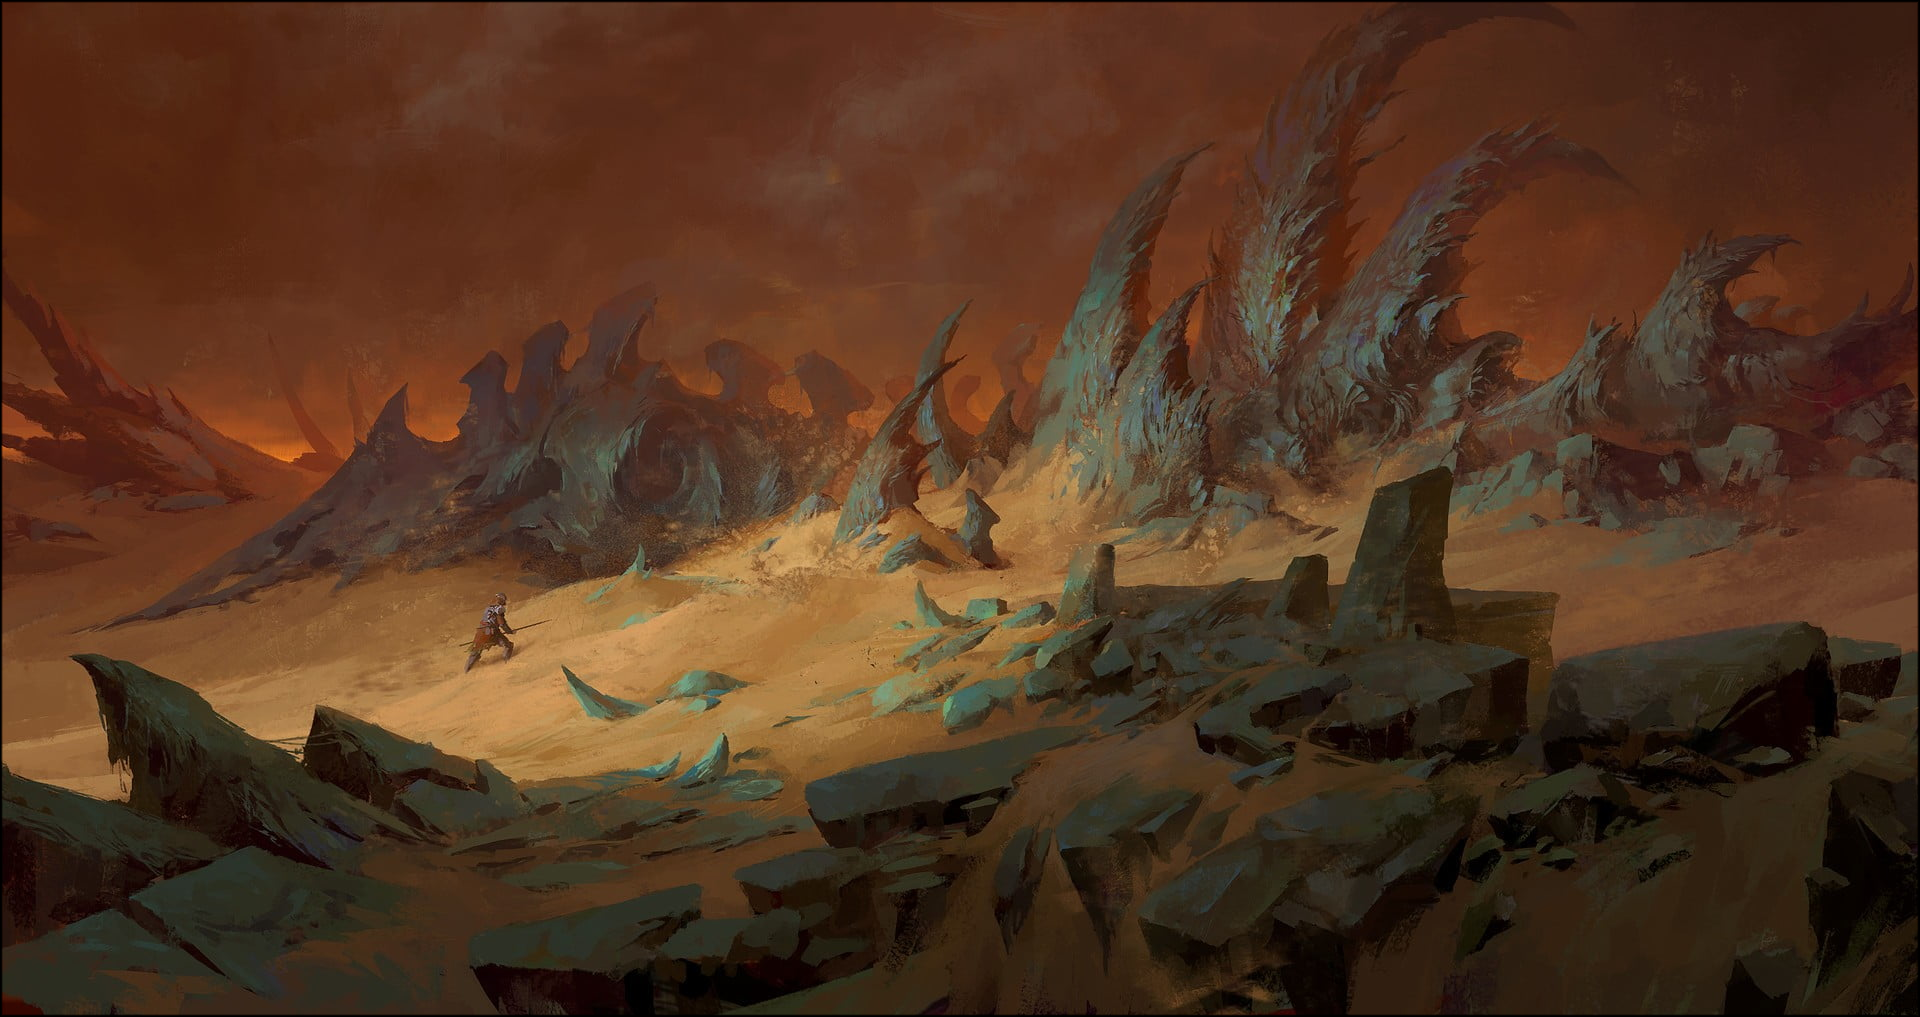
\includegraphics[width=0.95\textwidth]{01yuadrem/img/12dead_sea.png} \
%         \centering \large{\textbf{The Bone Cliffs of the Dead Sea}}
%     \end{DndTable}
% \end{table*}

\subsection*{The Three Deserts} \label{ssec::threedeserts}
Effectively splitting Yuadrem in half are the three deserts: Zoedrem, Zashlath, and the Dead Sea.

Zoedrem is a large expanse of yellow sands the embraces the waves of both the Whaler's Sea and the Teal Ocean.
The desert runs undisturbed from the Sulfur Lake down to the Defiled River.
It is commonly regarded as the most forgiving of the three deserts.

More fearsome than the sands are its inhabitants, the five dratl ird houses of Zoedrem.
Descendants of the fallen empire of Hulnar, they hide their settlements along the stone cliffs.
They are constantly in search of prey, robbing and murdering any traveler foolish enough to travel in their territories.

At the easternmost point of Zoedrem is the Sylvan Canyon, the only area in the desert able to host life.
The gorge is the home of the independent nation of Viphoger.
Apart from its inhabitants, the canyon's soil has rich natural deposits of oil, salt, and gemstones.
These resources grant Viphoger a strong economy despite its young age.

Southeast of Zoedrem and across the Ichor Mountains lie the Dead Sea, an artificial desert created by the tall kin's folly.
The desert's sands are of a sickly gray color, and any creature that inhabit the land for too long suffer particular mutations.
Its inhabitants, the treb gats and the cursed umans are perhaps the best examples of this.

The sands become blacker the more you approach the spire, the largest mountain in Yuadrem.
The et city of Jan'krug stands atop it, where the ritual that caused the Schism took place.
A long chasm divides the eastern region of the Dead Sea, remnants of the passage of the breathing island, Cabb Goem-Rlamesh.
Surrounded by hill, mountain, and river, the desert naturally prohibits passage to it, almost as if it's protecting a twisted secret.

Apart from the kins that call this desert home, the Dead Sea is infested with other monstrosities.
These are categorized into two: The Nyxborn and the children of Cabb.
The former are giant insect-like creatures that can be as large as an elephant and as precise as a mosquito.
The latter are tormented amalgamates that dislodged from Cabb Goem-Rlamesh, ever haunted by insatiable hunger and unending pain.

% Along with the tortles, grungs, and umans, the Schism brought forth terrible creatures known as the Nyxborn.
% These insect-like monstrosities can be as huge as the Mirmekolon, a colossal ant-lion hybrid, or as precise as the Khanokoladtes, a palm-sized moth that pierces skulls with its sharp dart-like mouth.

South, through the Hammerfall canyon, is the Zashlath desert, the driest of the three.
Featureless and white, only the hardy sunstruck oths have been able to call the desert home, and even they are wise enough to only establish by the neighboring mountains.

Zashlath practically receives no precipitation, and its white-colored sands reflect the scorching sunlight to deadly effect.
Truth is the desert remains largely unexplored to this date, and only rumors exist about the horrors that might hide among its sands.
Famous among these is the Haimorrois, a red horned snake whose bite forces the blood out of one's body.

% !TEX root = ../main.tex

\begin{figure}[t]
    \centering
    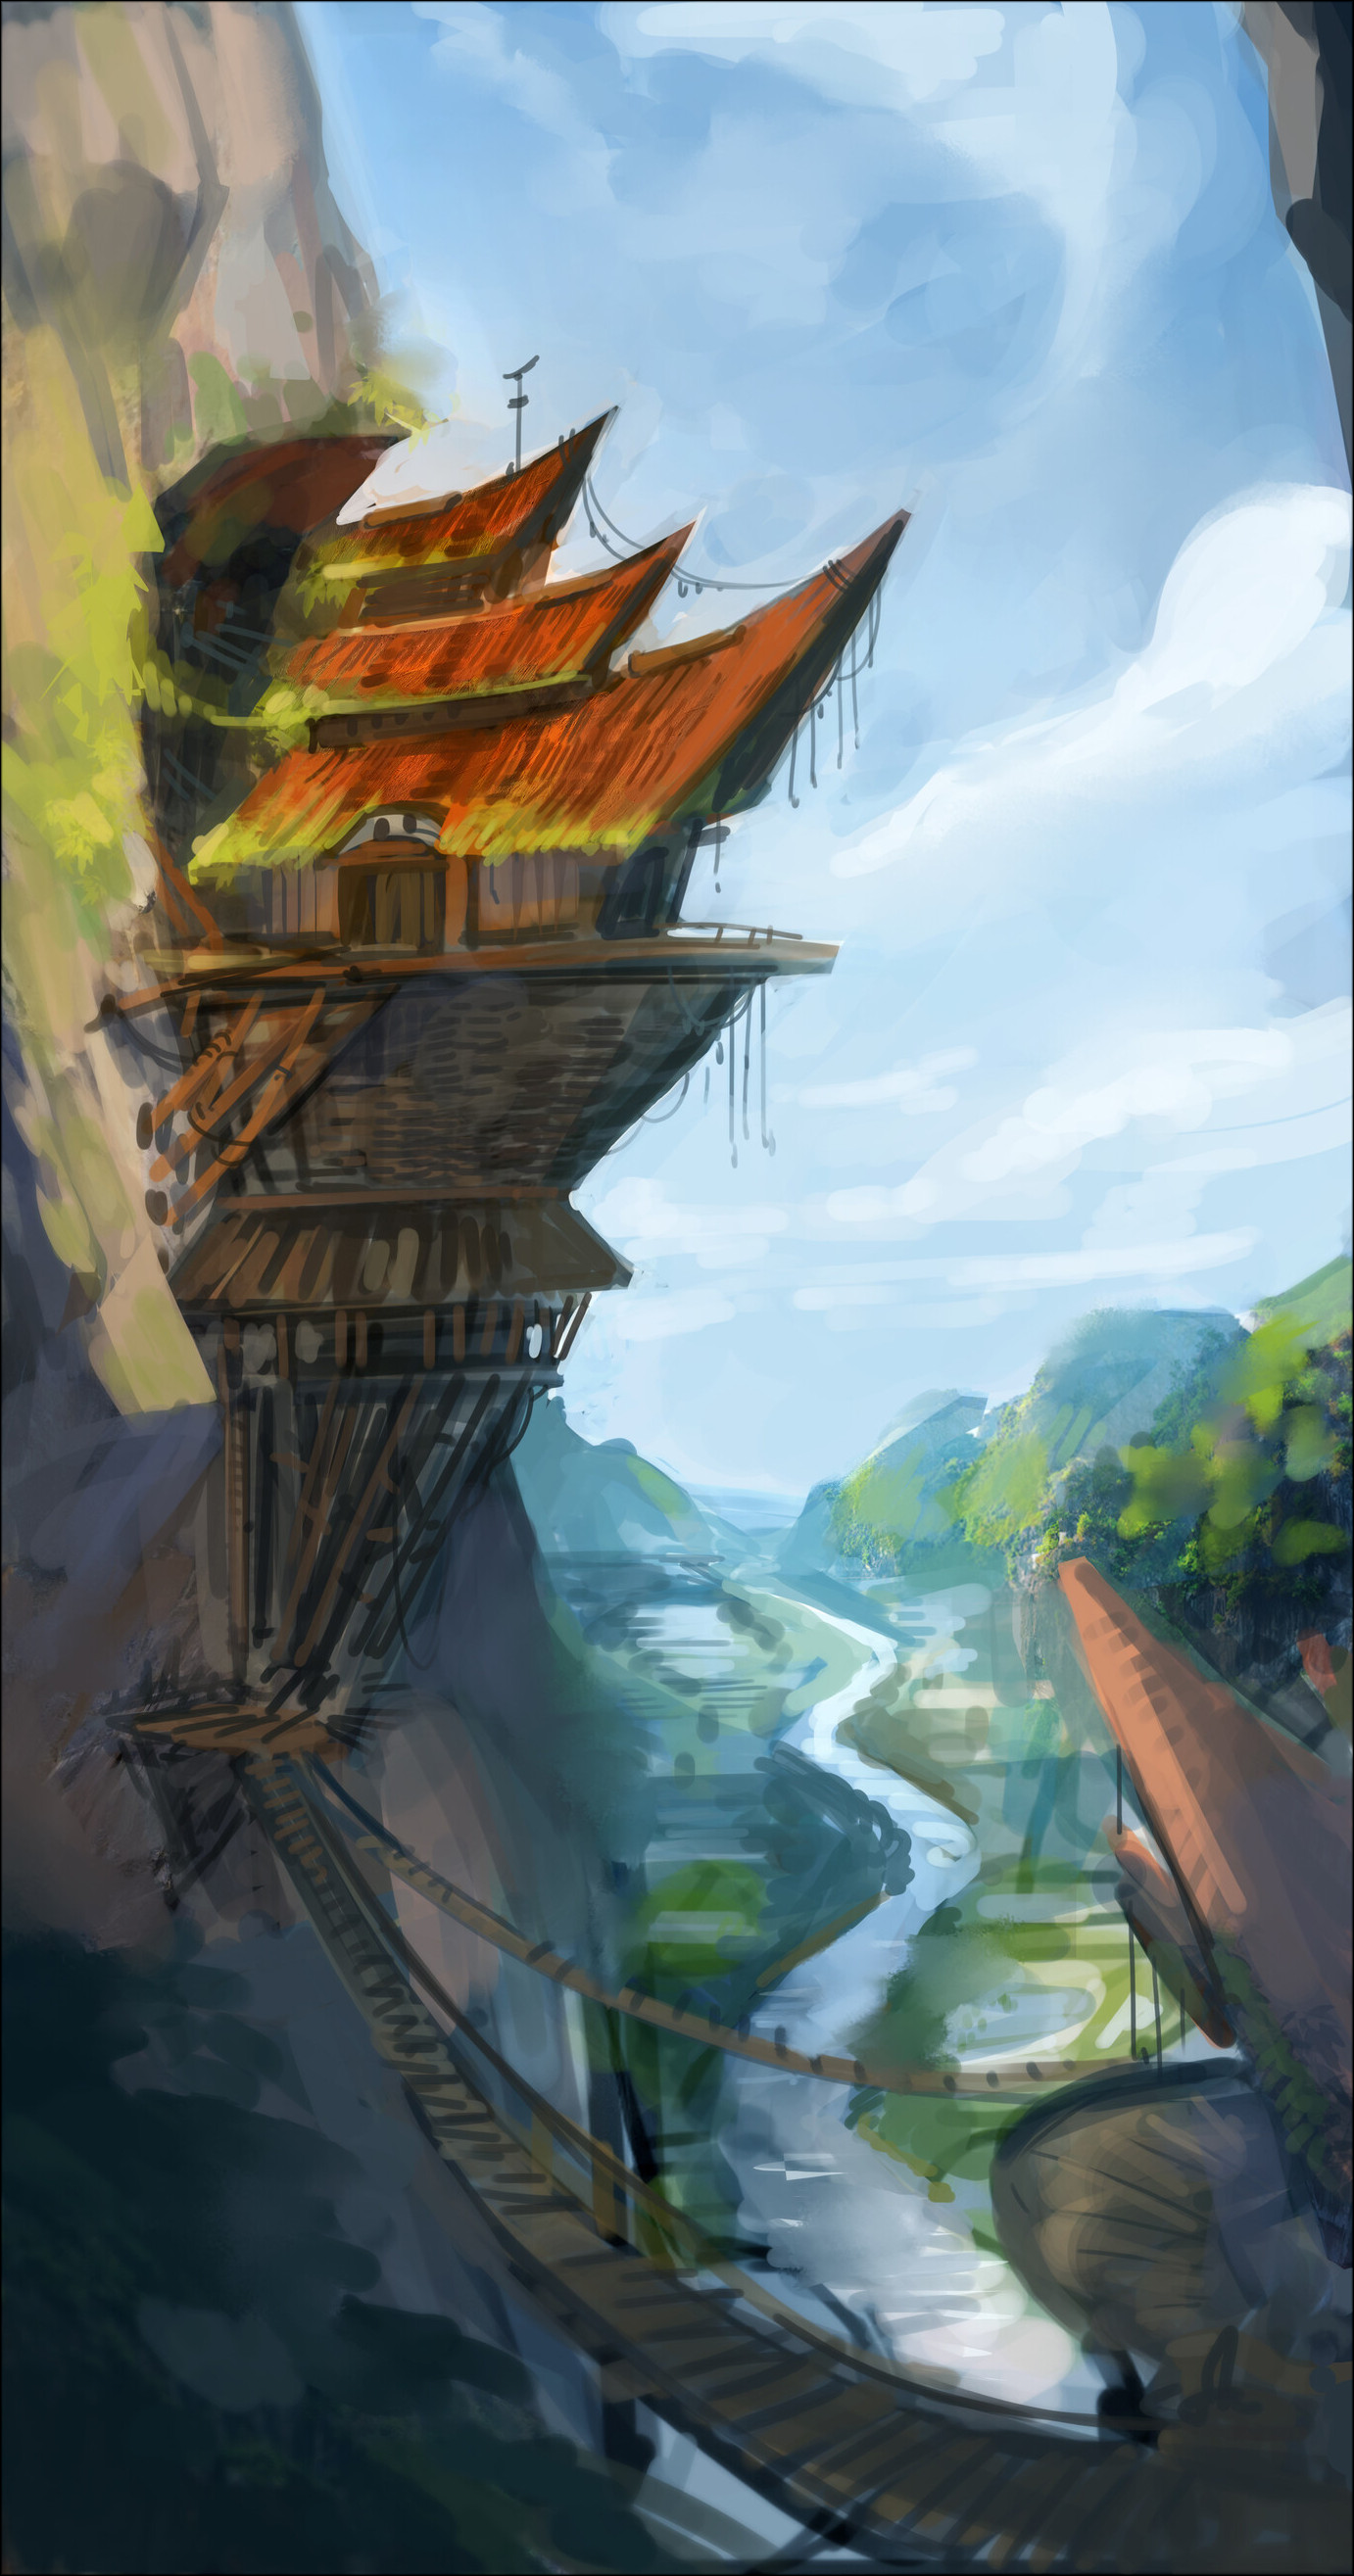
\includegraphics[width=0.46\textwidth]{01yuadrem/img/13siszgoel.png}
    \caption*{\centering \large{\textbf{Siszgoel, Kaldrathal's Capital}}} % TODO: Check if I can change the font of the caption
\end{figure}

\subsection*{Whaler's Sea} \label{ssec::whalerssea}

% intro
The cradle of modern civilization, the Whaler's Sea is home to both well-established and blooming countries.
Its coasts protected from harsh winds by mountain ranges and its cold waters supplied with both whale and idzel, the region couldn't be a better location to develop the modern world.
Idzels are large whale-like creatures known for their ship-sinking fury and their large supply of the valuable ambergris, the main ingredient in artificial qualars.

% Krejek and Kaljek
Sitting at the middle of the sea are the two southernmost islands of the Arctic Archipelago, Krejek and Kaljek.
The first is a large island covered by mountains, rocks plains, and deciduous forests.
It serves as the mainland for the independent nation of Kaldrathal.
%, who competes with Sulia as the main exporter of nitrate.

Starting out as a Krudzalian colony, they merged the quench-hardened steel of the thulkraka irds with their natural supply of nitrate.
This combination produces resilient steel firearms, including cannons, muskets, and flintlock handguns.
They remain the only exporter of these valuable weapons.

Kaljek, the smaller of the two islands, is a desolate land, with only few pine and birch forests.
It is separated by four nations inhabited by gat and ird alike.
While historically peaceful towards each other, they have recently been divided by conflict, all over the recently discovered gold veins that hide under their land.
% 661 AS: gold veins found under the ground.

% southern coast
South of both islands are the Horned Shores and the Fesh Peninsula.
The first is known for its calm, dry mediterranean climate, its sparse forests, and the great concrete gat city-states that rise from its ground.
Most of the land is devoid of natural resources, with scarce mines and low-quality wood.

% eastern coasts
East to these lands is the Fesh peninsula, an area inhabited mainly by gats, tortles and thulkraka irds.
A humid subtropical climate permeates the cape, and it is known for its harsh, capricious waters and frequent storms.
Also well-known are the tortles inhabiting the small island of Mbeat, for it is the only place where they have met safety after their arrival in Yuadrem.

In both regions lie the oldest nations of Yuadrem, the Seven kingdoms of the Sea.
Historically renowned raiders and pillagers, they are now famous for their passivity --- focusing on enterprise and artisanship.
What they offer is their expert craftgatship, and among them are the only bonecarvers capable of manufacturing qualars.

% western coast
Finally, to the west of Krejek one can find the two daughters of Palegna, the countries of Sulia and Drer.
The two nations were in a sense ``commisioned'' by the oth nation of Palegna.
Sulia was born to control the worrying growth of the Sulfur Lake, and Drer to restrict the growth of the bughna gat tribes of the Blank Fields.
% Both countries also served as an experiment of sorts for the word-obsessed oths, since the official language in both nations is the artificial Standard Language created by them.

Sulia benefited greatly from what would originally be their burden, and have developed a refined industry based on sulfur.
Their sulfur-based fertilizer is the basis of modern agriculture, their fiery blackpowder is only matched by Kaldrathal's, and their self-preserving wines are a taste craved all around the continent.
% They also have great sulfur-inlaid furniture!

Drer, in stark contrast with its sister, is a nation whose economy solely depends on pillage.
Re-imagining Sulia's blackpowder, they use their fire-bearing weapons to push back and raid their northern neighbors.

% !TEX root = ../main.tex
\subsection*{Beryl Sea} \label{ssec::berylsea}

The Beryl Sea is a searing, tropical region, ever battered by violent winds and waters.
The region is tapered in rainforests, and it houses two of the largest nations in Yuadrem: the warring Jenkashian empire and the mysterious Gannag.
The coasts see few other countries, and seldom do ships sail in these lands.
% Apart from the two, the coasts are also inhabited by a somewhat limited variety of countries, including the ancient Edede, the resilient Voskferm, and the strange Na'ane.

% Drejeck
Westernmost of Yuadrem is the thick, dark, and moist jungle of Drejeck.
Drejeck is the birthplace of the savage naenks and the ceremonial tsaneks, and is now entirely occupied by their nation, Gannag.
Despite being born even before the Schism, the beings of Gannag are primitive and untamed, and keep their tribal ways despite regular contact with more sophisticated cultures.
The jungle is also inhabited by large and dangerous beasts that threaten the unprepared explorer, like the aggressive nadubis or the silent whowie.
% And the bulettes and the Yara-ma-yha-who.

% Fog Gorge
East to Drejeck is the Fog Gorge, a well-forested canyon island ever enveloped in fog.
While primitive, the tribes of Gannag are far from free-living, and are bound by strong shackles to their superiors.
While naenks are used to this hierarchical system, many of the more intelligent tsaneks grow tired of it over time.
A hundred and fifty years ago, a group of tsaneks went as far as to establish their own independent tribe of Na'ane in the misty island, abandoning their brethren in favor of an unrestrained lifestyle.
Freely they carry on with their ceremonies and rituals, protected from their neighbors by mist and stone.

% Qul archipelago
Further east one finds the Qul archipelago, a clump of islands that collectively served as the birth bed of the Jenkashian empire.
Jenkash is a coalition of tribes that only managed to unite after cutting down the last tree in their mountainous islands.
This led to an explosive expansion of their empire, and they swiftly conquered the neighboring lands.
Their territories now span most of the coasts of the Beryl Sea.

The archipelago itself is absolutely desolate, with barely any tree or foliage growing atop its igneous rock.
Perhaps the only bright side of this uncontrolled deforestation is the fact that it brought to light the iron and diamond veins in the eastern side of the archipelago.
These resources are heavily exploited by the qulbaba irds, and led to their signature diamond daggers.

% Dratl'fal savanna
North of the archipelago is the Dratl'fal savanna, occupied entirely by Jenkash.
The only plant that freely grows in the savanna is bafarmat, a purple moss covering its entire southeastern coast.
This plant is the primary food source of the cavernous species that live under the ichor mountains.
Its spread has allowed the hornbeetles to move into the area, a strong species of giant blue beetles that served as companions to the now ruined nation of Phrisht.

In oldentimes, the dry lands served as the birth bed for many gat city-states, of which only Dzorvepem and Jorea remain standing, now part of Jenkash.
Despite its lack of resources, the whole area was sought after by the now divided empire of Hulnar, who battled against the blooming nation of Phrisht for more than 300 years for it.
This everlasting conflict was only stopped by Jenkash, who in their thirst for conquest ended up dissolving the untiring countries.

% \begin{figure}[t]
%     \centering
%     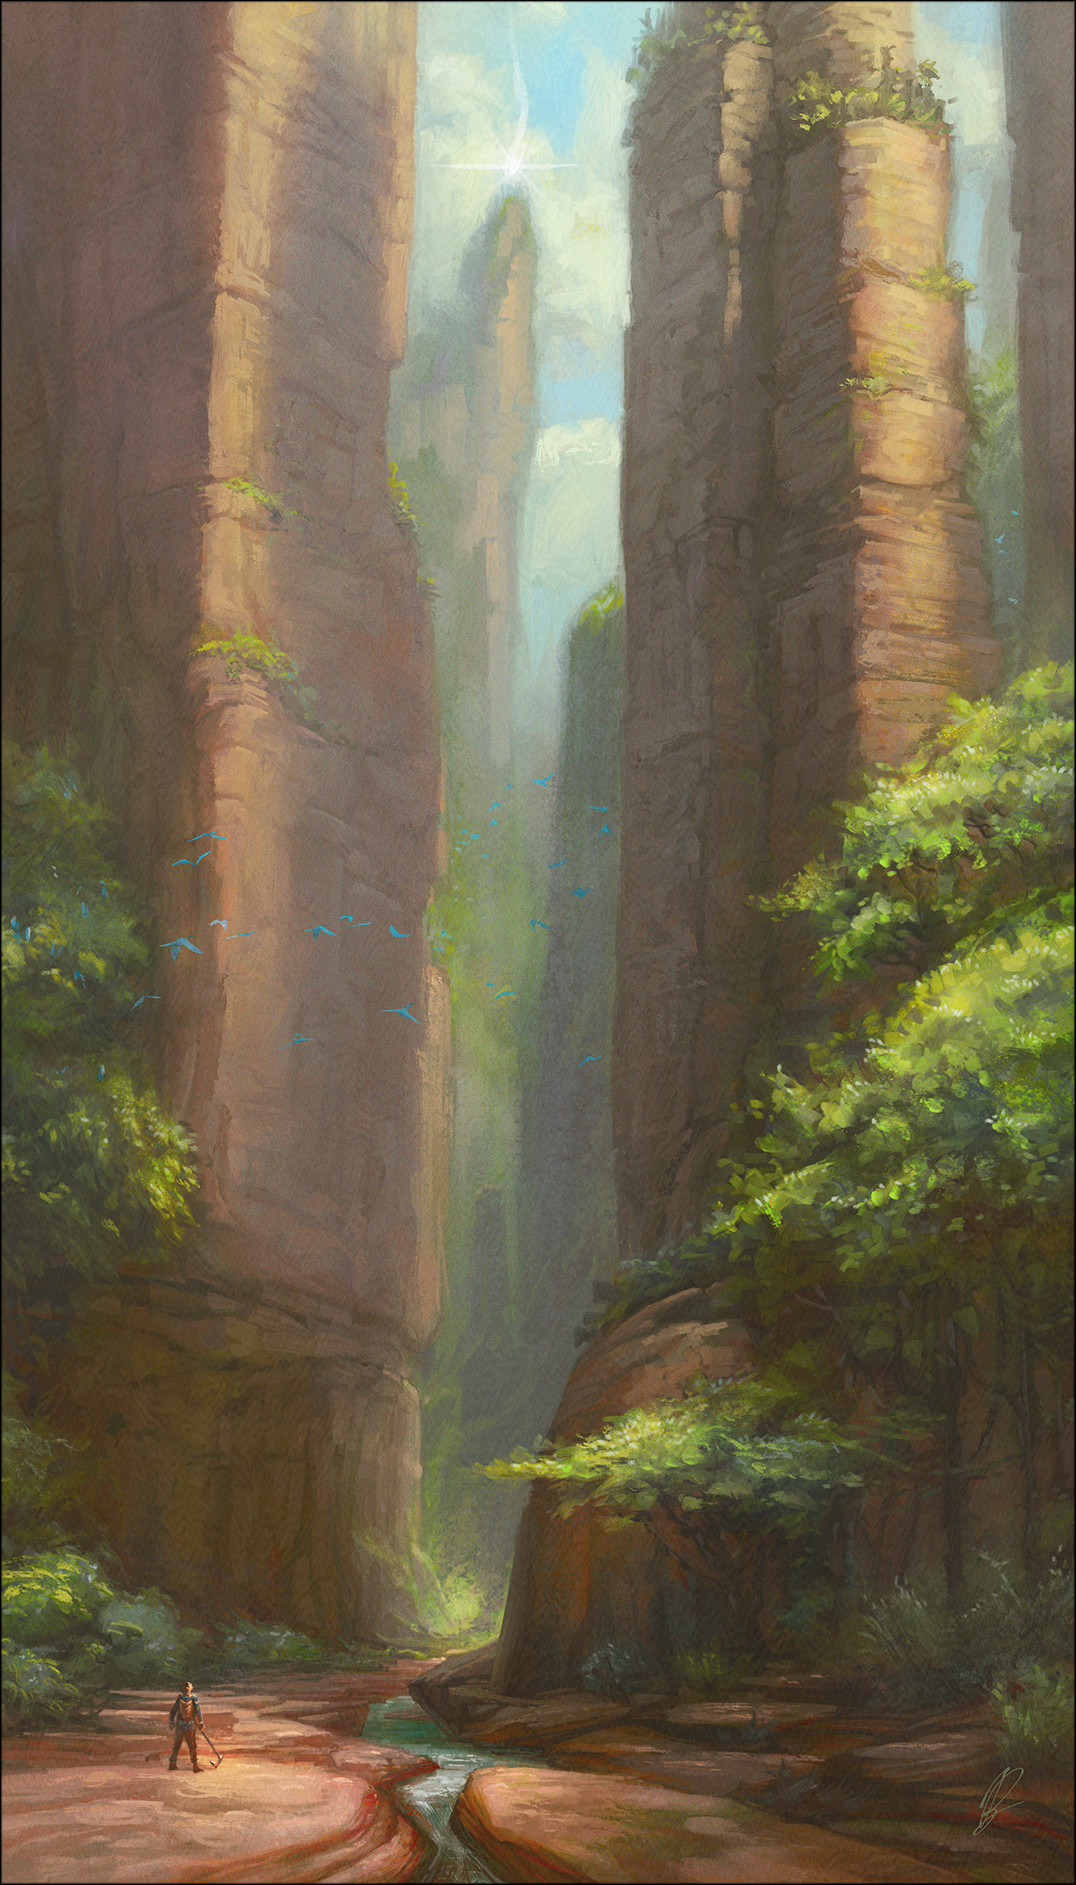
\includegraphics[width=0.46\textwidth]{01yuadrem/img/14fog_gorge.png}
%     \caption*{\centering \large{\textbf{The Fog Gorge}}}
% \end{figure}

% Ironlakes Island & Zashlath savanna
Moving to the easternmost portion of the sea one can find the Ironlakes Island and the Zashlath savanna.
The former is a large island full of forests and lakes.
It was historically a part of the peaceful marset nation of Edede, but most of it now belongs to the warring empire.
The Zashlath savanna is the area west of the desert, protected from its dry air by the moisture of the cerulean waters.

% !TEX root = ../main.tex

\begin{table*}[b]%
    \begin{DndTable}[width=\linewidth]{X}
        \centering
        \includegraphics[width=0.98\textwidth]{01yuadrem/img/15om.png} \
        \centering \large{\textbf{Om, Isken's Capital}}
    \end{DndTable}
\end{table*}

\subsection*{Barbaric Territories} \label{ssec::barbaricterritories}

To the east of Yuadrem are the Barbaric Territories, a region defined by the brutality of war and the greed of an empire.
From north to south, the land can be divided into five areas, each with its own distinct characteristics: the Drylands, Cabb Goem-Rlamesh, the Shield Sea, the Chirping Wilds, and the Xuam Peninsula.

% Drylands
Northernmost are the Drylands, a field devoid of trees or any sort of tall flora.
The area is plain and parched, dried over the years for its lack of rains or rivers.
The northernmost area of the savanna remains bare to date, and is the most tortuous stretch between the Fesh Peninsula and the southern nations.

% Mzavit river and southern savanna
Down across the Mzavit River, the savanna becomes humid and with this water comes civilization.
A wide array of gat city-states have been established here.
Able to withstand the thunderous force of the Jenkashian and Iskenese armies and the hulking chimeras from the Next, these states are noteworthy for their fortitude.
Of special note is the adamant country of Byurev, who have halted the growth of Isken for almost three centuries.

% Cabb Goem-Rlamesh
% NOTE: In the whole island of Cabb Goem-Rlamesh a faint crying sound can be heard.
Off the coast of the Drylands lies a place known as the breathing island, Cabb Goem-Rlamesh.
A harrowing immensity, the landmass is constructed entirely of flesh and bone, and is believed to be what remains of the ets.
Not much is known about the island, and none of the few explorers who have travelled to it retain their sanity.
The mad tell tales of a mortifying city of flesh, and of strange, shape-shifting inhabitants.

% Shield Sea & The Nest
% Wrong information - geomancy was invented by an ancient civilization that warred with the tall kin eons ago, but was erased from history by the victors. There are ruins from this civilization at the basin of the lake, and Fo is the last remaining member from it.
Southwest of the Drylands rest the Shield Sea, an enormous body of water fed by a wide array of tributaries from the Forking Peaks.
In antiquity, the ruined ird civilization of Hairuus invented the art of geomancy in its coasts, raising from the basin the island of ``The Nest'' at its center.
The island currently hosts only one being, Fo.
Fo is a strange creature, rumored to be out of this world.
It welcomes visitors with a variety of fierce chimeras.

% Chirping Wilds
Southeast from the Drylands and passing through the Do Nana swamp are the Chirping Wilds, a vast and largely untamed rainforest.
The jungle is inhabited only by the Iskenese empire, a large grung nation that expelled the original ird and marset population.
The only territories currently not held by the grungs' military might are the strong qulbaba irds of Harual to the west, and the marsets of Uzuz from the Xuam peninsula.

The Xuam Peninsula is the southermost point of the Barbaric Territories, and is located just south of the Grasping Gulf.
The region has facilitated the development of Uzuz due to the heavy presence of wurmroot, a white-leaf poplar tree that is conveniently toxic to all foreigner kins, specially to grungs.

% !TEX root = ../main.tex

% \begin{table*}[t]%
%     \begin{DndTable}[width=\linewidth]{X}
%         \centering
%         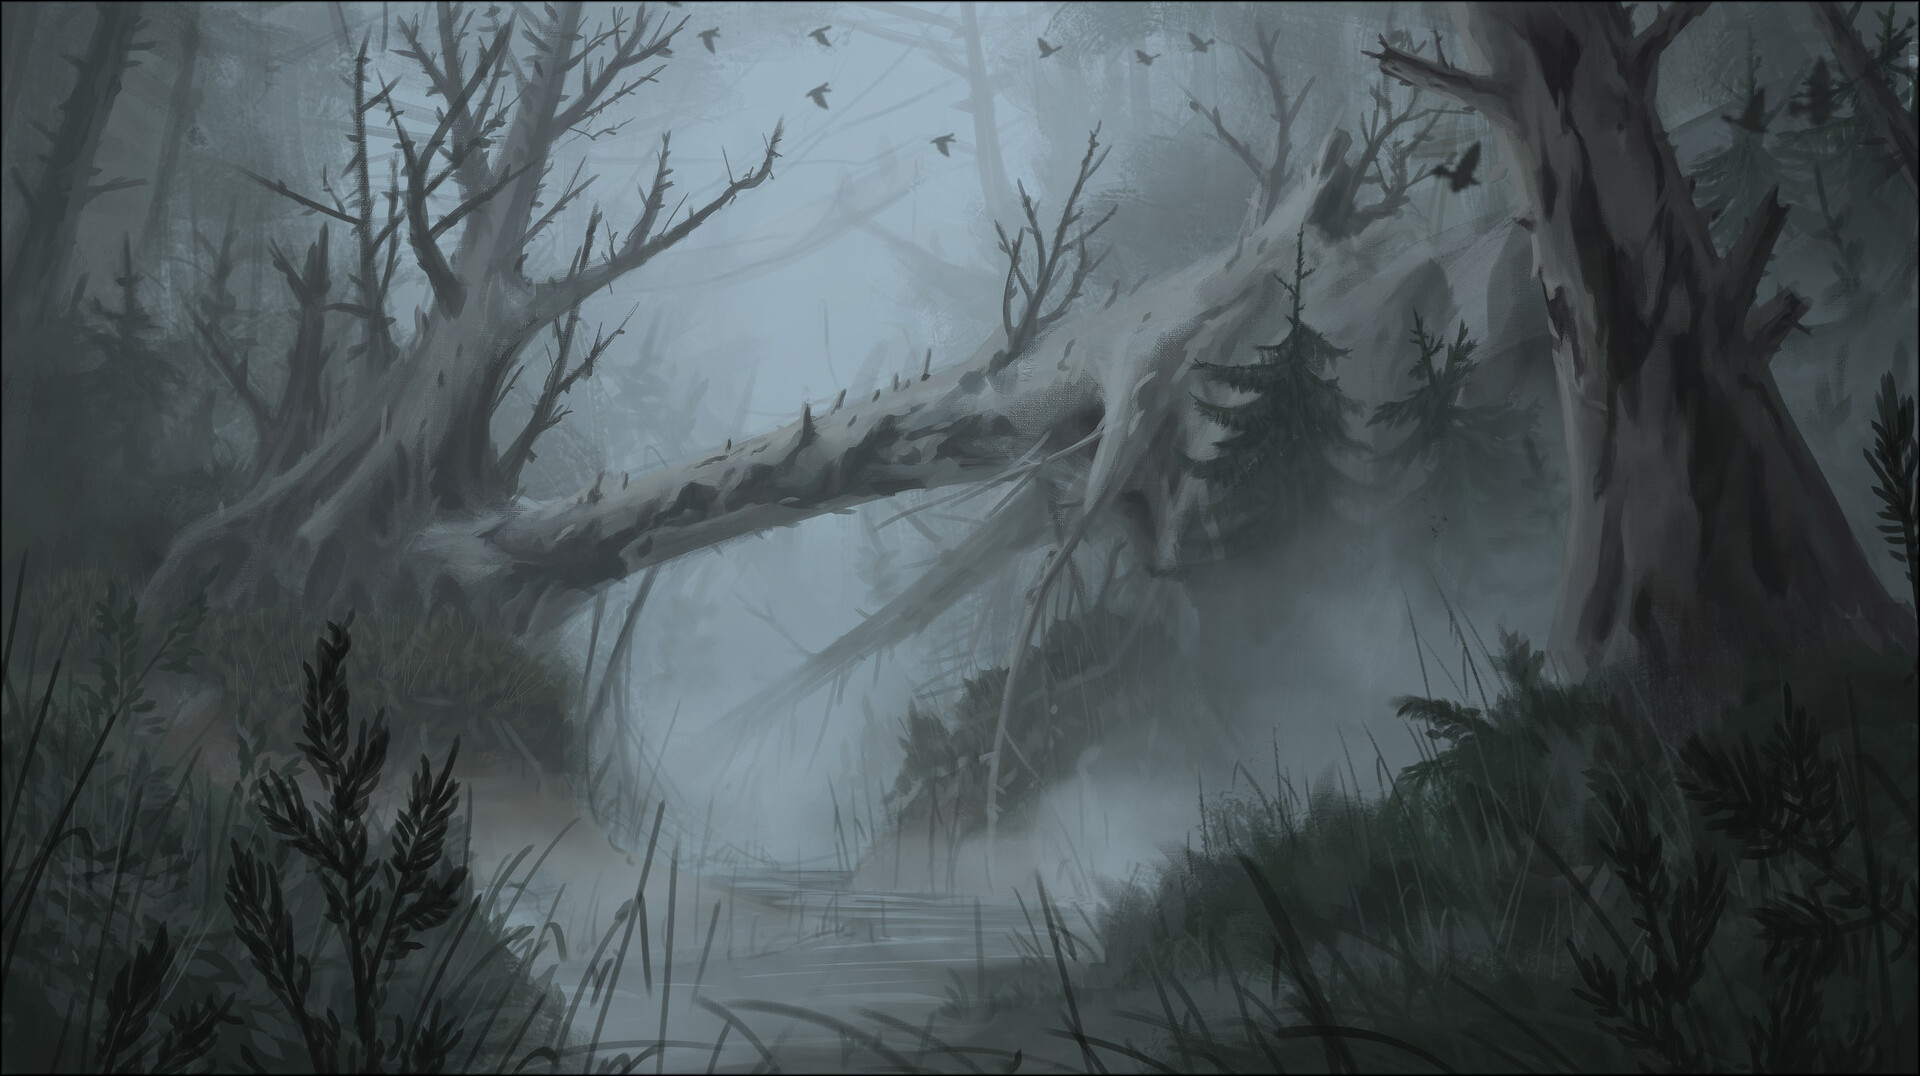
\includegraphics[width=0.98\textwidth]{01yuadrem/img/16pale_blemish.png} \
%         \centering \large{\textbf{Forests Surrounding the Pale Blemish}}
%     \end{DndTable}
% \end{table*}

\subsection*{Wildlands} \label{ssec::wildlands}

% intro
The southernmost region of Yuadrem is aptly named the Wildlands, for it is a large expanse of untamed fields, forests, and lakes.
Starting at the bottom-most part of the forking peaks, the area has seen very little intervention from the civilized world.
This is attributed to the fact that the Wildlands are infested with both deadly creatures and strange tide-altering illnesses.

% Savage Plains
Just below the forking peaks and the Beal river is the northmost point of the Wildlands, the Savage Plains.
They are a humid subtropical area covered by marshes and plains, with few patches of forest in-between.
Fed by many rivers from the mountains, the lands define the southern territories of the Iskenese empire, expanding thorough the whole region.

However, Isken's grip on the Savage Plains is tenuous at best, as the region is as much controlled by the grungs as it is by the local wildlife.
Just as in the forest below, a great variety of foul beasts and creatures can be found in these swamps.
Of special note among these are the giant mole-like jinshus, beasts unique to region who suffocate the unprepared by sinking them beneath the earth.

% Everwoods
As dangerous as these plains are the Everwoods, the forest that grows south of them.
This ancient woodland used to be a place of respite after the harsh swamps, but all that swiftly changed about 400 years ago.
In an attempt to manipulate the tides, the Rashiist school of thought from Ignelli summoned The Sorrow into Yuadrem.
The Sorrow is an entity of unknown origin, who seeped into Yuadrem due to the Rashiists folly.
On arrival, it swiftly slayed all members of the school of thought, and brought fourth with it strange creatures and diseases that now plague the once peaceful forest.
This event came to be known as the Tidal Sway.

% Pale Blemish
Not only bringing forth pain and disease, the Tidal Sway also ravaged the land around Ignelli, area now known as the pale blemish.
All flora was destroyed, and the ground turned into badlands.
The field now serves as a grim reminder to all of the dangers of manipulating the tides.

Despite the destruction, the scholars from the Igneist school continue to work in their temple, studying the tides and The Sorrow.
Perhaps one day they'll achieve their goal and undo their sister school's sins, expelling the Sorrow and healing their lands.

% Niknek Peninsula
West of the Everwoods is the Niknek peninsula, a thin, elongated stretch of land filled with volcanoes and gorges.
The cape was spared from most of the effects of the Tidal Sway.
Niknek and the nearby Vuvu Isles now house the refuge marsets from the Ironlakes Island.

% Elderberry Wilds
At the southern tip of Yuadrem are the Elderberry Wilds and the Ironwoods, a set of pine and spruce forest surrounding the Manta Sea.
The area is partly occupied by Gronselar, an old and forgotten colony of Krudzal.
% Not much is known about these forests due to their remote location.
% Not much is known about the area due to its remote location, but even here a semblance of civilization exists. in the form of the ird nation of Gronselar, and the regions of Froibias, Glameas, and Visilias.

